\documentclass[a4paper]{article}

\usepackage[english]{babel}
\usepackage[utf8]{inputenc}
\usepackage[titletoc, toc]{appendix}
\usepackage{amsmath}
\usepackage{graphicx}
\usepackage{mdframed}
\usepackage{cancel}
\usepackage{caption}
\usepackage{lipsum}
\usepackage{listings}
\usepackage{float}
\usepackage[colorinlistoftodos]{todonotes}

\title{Uncertainty Quantification (ACM41000) \\ Mini Project 1}

\author{Ian Towey \\ \\ 04128591}

\date{\today}

\lstdefinestyle{custom_py_style}{
  belowcaptionskip=1\baselineskip,
  breaklines=true,
  frame=L,
  xleftmargin=\parindent,
  language=Python,
  showstringspaces=false,
  basicstyle=\footnotesize\ttfamily,
  keywordstyle=\bfseries\color{green!40!black},
  commentstyle=\itshape\color{purple!40!black},
  identifierstyle=\color{blue},
  stringstyle=\color{orange}
}

% Number the subsubsections and include them in the TOC
\setcounter{secnumdepth}{3}
\setcounter{tocdepth}{3}
\setcounter{section}{-1}

\newenvironment{aside}
  {\begin{mdframed}[style=0,%
      leftline=false,rightline=false,leftmargin=2em,rightmargin=2em,%
          innerleftmargin=0pt,innerrightmargin=0pt,linewidth=0.5pt,%
      skipabove=7pt,skipbelow=7pt]\footnotesize}
  {\end{mdframed}}

\begin{document}

  \maketitle

  \begin{abstract}
    Analytic and numerical analysis of a basic SIR epidemic model
  \end{abstract}

\tableofcontents
\newpage

\section{Introduction}
\label{sec:introduction}
This report presents analysis of a SIR epidemic model on a fixed population of size $N$. \\

The population is split into 3 groups susceptible, infected and recovered, $x(t)$, $y(t)$ and $z(t)$ 
respectively.

\begin{align}
 x(t) + y(t) + z(t) &= N
\end{align}
The set of equations to model the different population subgroups are:
\begin{subequations}
\begin{align}
  \frac{\mathsf{d}x}{\mathsf{d}t} &= -kxy			\\
  \frac{\mathsf{d}y}{\mathsf{d}t} &= kxy - ly		\\
  \frac{\mathsf{d}z}{\mathsf{d}t} &= ly			
\end{align}
\end{subequations}

\section{Analytic analysis \textit{x}- and \textit{y}- equations alone}
\label{sec:theory}
From Equation (2a)

\begin{align}
   y &= \frac{1}{l}\frac{\mathsf{d}z}{\mathsf{d}t}		
\end{align}
Substituting Equation (3) into Equation (2a) and solving for $x(t)$:
\begin{align*}
  \frac{\mathsf{d}x}{\mathsf{d}t} &= -\frac{kx}{l}\frac{\mathsf{d}z}{\mathsf{d}t}	\\		
  \frac{\mathsf{d}x}{x} &= -\frac{k\mathsf{d}z}{l}		\\
  \int{\frac{\mathsf{d}x}{x}} &= -\frac{k}{l}\int{\mathsf{d}z}	\\
  \ln(x) &= -\frac{kz}{l} + C			\\
  x(t) &= e^{-\frac{kz}{l}}e^{C}
\end{align*}
Letting $e^{C} = x_{0}$ gives
\begin{align}
  x(t) &= x_{0}e^{-\frac{kz}{l}}
\end{align}


\section{Solve fot y(t)}

\begin{align*}
  \frac{\mathsf{d}y}{\mathsf{d}t} &= kxy - ly						\\
  \frac{\mathsf{d}y}{\mathsf{d}t} &= - \bigg(\frac{\mathsf{d}x}{\mathsf{d}t} + \frac{\mathsf{d}z}{\mathsf{d}t}\bigg)	  	\\
  \mathsf{d}y &= - \bigg(\mathsf{d}x + \mathsf{d}z\bigg)	  					\\
  \int{\mathsf{d}y} &= - \bigg(\int{\mathsf{d}x} + \int{\mathsf{d}z}\bigg)	  			\\
  y(t) &= - x(t) - z(t) + C						\\
\end{align*}
From Equation (1), we can see that $C = N$, giving:
\begin{align*}
  y(t) &= - x(t) - z(t) + N						
\end{align*}
Substituting RHS of Equation (6) for $x(t)$ yields: 
\begin{align}
  y(t) &= N - x_{0}e^{-\frac{kz}{l}} - z(t)
\end{align}

\section{Quick view of $\frac{\mathsf{d}z}{\mathsf{d}t}$}
\begin{align*}
  \frac{\mathsf{d}z}{\mathsf{d}t} &= ly			
\end{align*}
Substituting RHS of Equation (7) in for $y(t)$, yields:
\begin{align}
    \label{xxx}
    \frac{\mathsf{d}z}{\mathsf{d}t} &= l[N - x_{0}e^{-\frac{kz}{l}} - z(t)]			
\end{align}

Equation (\ref{xxx}) is an ODE with a single dependent variable $z$ and 4 independent constants , $l, k, N, x_{0}$. While this could probably be analyzed using qualitative analysis such as finding fixed points and testing the stability
of these fixed points, doing so would not be easy due to the number of independent constants and their impact on this analysis.

\section{Rescaling to reduce the number of constants}
Using variable transforms
\begin{center}
  $(i) \hspace{5pt} u = \frac{kz}{l};  \hspace{35pt} (ii) \hspace{5pt} a = \frac{N}{x_{0}};  \hspace{35pt} (iii) \hspace{5pt} b = \frac{l}{kx_{0}}; \hspace{35pt} (iv) \hspace{5pt} \tau = kx_{0}t$
\end{center}

\begin{align*}
  \frac{\mathsf{d}z}{\mathsf{d}t} &= l[N - x_{0}e^{-\frac{kz}{l}} - z(t)]						\\
  \frac{1}{x_{0}}\frac{\mathsf{d}z}{\mathsf{d}t} &= l[\frac{N}{x_{0}} - e^{-\frac{kz}{l}} - \frac{z}{x_{0}}]	\\		
  \frac{1}{x_{0}}\frac{\mathsf{d}z}{\mathsf{d}t} &= l[a - e^{-\frac{kz}{l}} - \frac{z}{x_{0}}]			
\end{align*}
From $(i)$ above, $z = \frac{ul}{k}$:
\begin{align}
  \frac{1}{x_{0}}\frac{\mathsf{d}z}{\mathsf{d}t} &= l[a - e^{-\frac{\bcancel{k}u\bcancel{l}}{\bcancel{k}\bcancel{l}}} - \frac{ul}{kx_{0}}]			
\end{align}
From $ (iii) \hspace{5pt} b = \frac{l}{kx_{0}}$:
\begin{align}
  \frac{1}{x_{0}}\frac{\mathsf{d}z}{\mathsf{d}t} &= l[a - e^{-u} - bu] 			
\end{align}

\begin{aside}
  \begin{align*}
     u = \frac{kz}{l} \Longrightarrow \mathsf{d}u = \frac{k \mathsf{d}z}{l} \Longrightarrow \mathsf{d}z = \frac{l \mathsf{d}u}{k}	
  \end{align*}
  \begin{align*}
     \tau = kx_{0}t \Longrightarrow \mathsf{d}\tau = kx_{0}\mathsf{d}t \Longrightarrow \mathsf{d}t = \frac{\mathsf{d}\tau}{kx_{0}} 
  \end{align*}
  Using the above definitions for $\mathsf{d}z$ and $\mathsf{d}t$ to find ratio of $\frac{\mathsf{d}z}{\mathsf{d}t}$
  \begin{align*}
     \frac{\mathsf{d}z}{\mathsf{d}t} = \dfrac{l \mathsf{d}u}{k} \dfrac{\quad 1 \quad}{\dfrac{\mathsf{d}\tau}{kx_{0}}} =  \dfrac{l \mathsf{d}u}{\bcancel{k}} \dfrac{\bcancel{k}x_{0}}{\mathsf{d}\tau} = l x_{0} \frac{\mathsf{d}u}{\mathsf{d}\tau}
  \end{align*}
\end{aside}
Substituting for $\frac{\mathsf{d}z}{\mathsf{d}t}$ into Equation (8):
\begin{align*}
  \frac{1}{\bcancel{x_{0}}}\bcancel{l} \bcancel{x_{0}}\frac{ \mathsf{d}u}{\mathsf{d}\tau} &= \bcancel{l}[a - e^{-u} - bu] 			
\end{align*}
Yields the desired equation
\begin{align}
  \frac{\mathsf{d}u}{\mathsf{d}\tau} &= a - e^{-u} - bu 			
\end{align}

\section{Fixed points / stability analysis of $\frac{\mathsf{d}u}{\mathsf{d}\tau}$}

\begin{align*}
  \frac{\mathsf{d}u}{\mathsf{d}\tau} &= a - e^{-u} - bu 			
\end{align*}
\begin{align*}
  f(u) &= a - e^{-u} - bu 							
\end{align*}

Analyzing $f(u)$ at zero, $f(0) = a - e^0 - b0 = a - 1 \geq 0$, 
\begin{itemize}
 \item if $a = 1$ , then $f(0) = 0$, this is the trivial fixed point which represented when there are no infected people in the system initially, as $a = N/x_{0} = (x_{0} + y_{0})/x_{0} = 1$, therefore N = $x_{0}$ 
 \item if $a > 0$, then $f(0) > 0$, therefore $a = N/x_{0} = (x_{0} + y_{0})/x_{0} > 1$ and $y_{0} > 0$ indicates there are some infected people in the system at $t_{0}$.
\end{itemize}

Analyzing $f(u)$ as $u\to\infty$ 
\begin{align}
  \label{b_anal}
  \lim_{u\to\infty} f(u) = \lim_{u\to\infty} [a - e^{-u} - bu] = -bu									
\end{align}
\begin{itemize}
 \item As $u$ grows large the linear terms $-bu$ dominates and the equation looks like a stright line as show in Figure (\ref{fig:fp_diff_ab}). 
\end{itemize}

\begin{figure}[H]
\centering
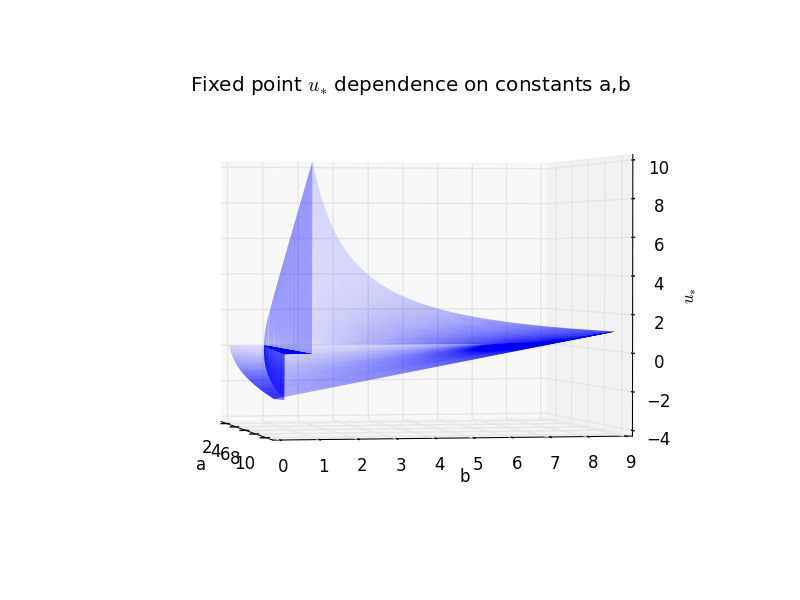
\includegraphics[width=1\textwidth]{3D_plot.png}
\caption{\label{fig:3d}$u_{*}$ vs $a$ vs $b$}
\end{figure}

Figure (\ref{fig:3d}) shows a 3D plot of $u_{*}$ for a range of values for $a$ and $b$, 

\newpage

\section{Analysis of parameter $b$}
From Equation (\ref{b_anal}), we can see the value of parameter $b$ dominates for large values of $u$. To find the single maximum analytically we solve $f'(u_{*}) = 0$

\begin{align*}
  f'(u_{*}) &= e^{-u_{*}} - b = 0 							
\end{align*}
\begin{align*}
  u_{*} &= -ln(b) 							
\end{align*}

Checking the sign of the second derivative $f''(u) = -e^{-u} < 0$ for all $u$ , so $u_{*} = -ln(b)$ is a maximum.
$f(u)$ has one fixed point $u_{*}$, and from Figure (\ref{fig:fp_diff_ab}) and (\ref{fig:df}) this is a stable fixed point.

\begin{figure}[H]
\label{yyy}
\centering
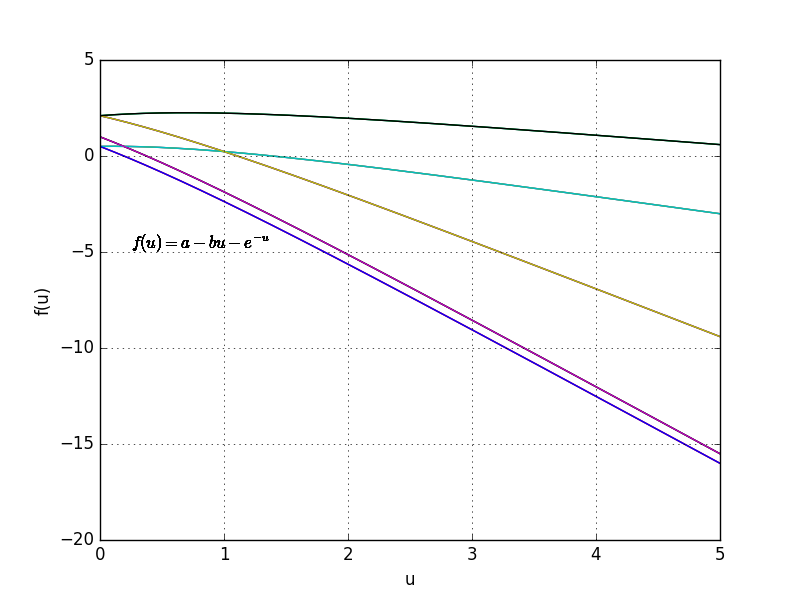
\includegraphics[width=1\textwidth]{fp_diff_ab.png}
\caption{\label{fig:fp_diff_ab}Fixed point $U_{*}$, for different values of $a$ and $b$.}
\end{figure}

Figure (\ref{fig:df}) shows a screen shot of the interactive \textit{maxima} plot with sample trajectory paths (these can be generated by just tapping on the plot with cursor and using the sliders to chnage the values of $a$ and $b$) 

\begin{figure}[H]
\centering
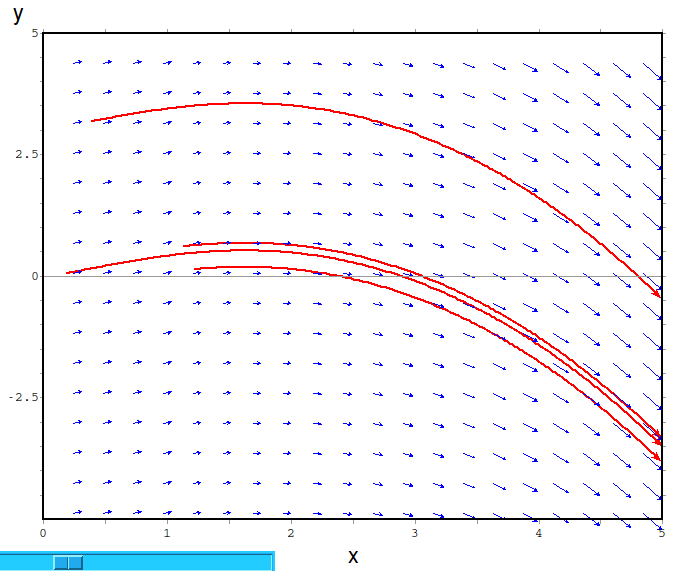
\includegraphics[width=1\textwidth]{df.png}
\caption{\label{fig:df}direction field of $f(u)$}
\end{figure}

\section{Numerically solutions}

The Python package \textit{scipy} and specifically the \textit{integrate} function were used to solve the Equation (11) numerically for various
values of $a$ and $b$. Figures 3 - 8 graphically show the evolution of the infections for a few representative values of $a$ and $b$.

\begin{center}
  \begin{tabular}{ | c || c | c | c | c |}
    \hline
    \multicolumn{5}{|l|}{Population N = 1000} \\
    \multicolumn{5}{|c|}{} \\
    \hline
	       & $a$ & $b$ & $x_{0}$ & $y_{0}$ 	\\ \hline 
    Figure (3) & 1.5 & 0.9  & 6666.66 & 3333.33 \\ \hline
    Figure (4) & 2   & 3.5  & 5000    & 5000 	\\ \hline
    Figure (5) & 3.1 & 2.5  & 3225.8  & 6774.19 \\ \hline
    Figure (6) & 3.1 & 0.5  & 3225.8  & 6774.19 \\ \hline
    Figure (7) & 1.5 & 3.5  & 6666.66 & 3333.33 \\ \hline
    Figure (8) & 1.1 & 0.01 & 9090.9  & 909.09 	\\ \hline
    \hline
  \end{tabular}
\end{center}

From the plots the significance of the parameter $b$ is evident. For values of $b < 1$, the number of infected increases small values of $\tau$
before decaying to $0$, with the decay rate increasing as b gets larger in size. When $b > 1$, the number of infected decreases forall $\tau$.

The smaller the value of $b$ the faster the rate if infection is and the slower the rate of recovery is as can be seen in Figure 8.

\begin{figure}[H]
\centering
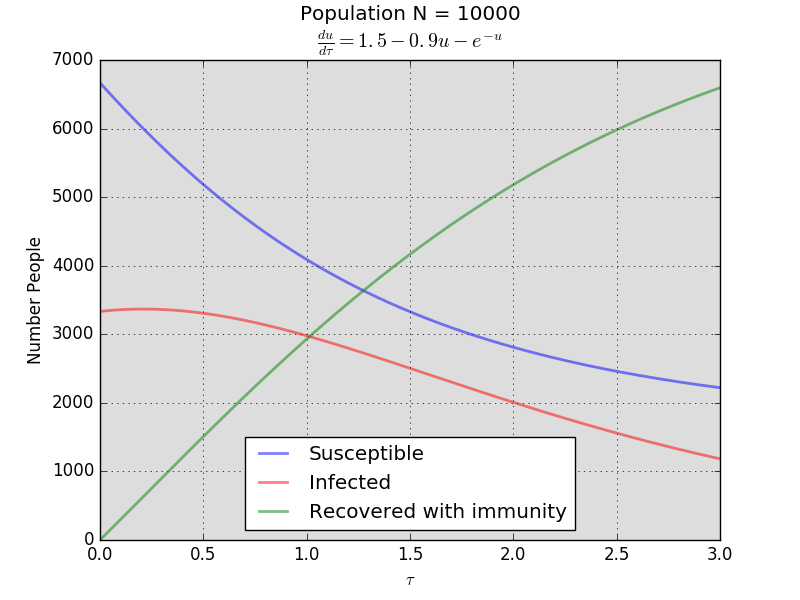
\includegraphics[width=1\textwidth]{q7_1.png}
\caption{\label{fig:data}Todo}
\end{figure}
\begin{figure}[H]
\centering
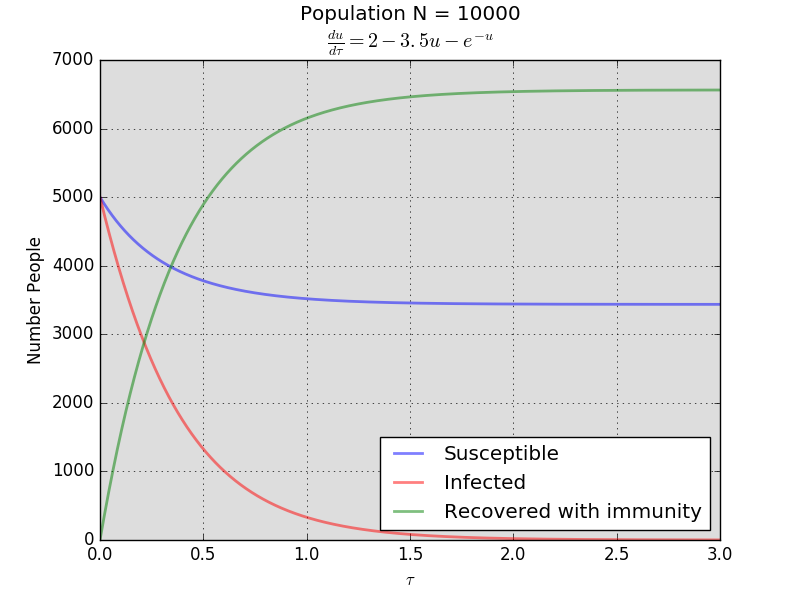
\includegraphics[width=1\textwidth]{q7_2.png}
\caption{\label{fig:data}Todo}
\end{figure}
\begin{figure}[H]
\centering
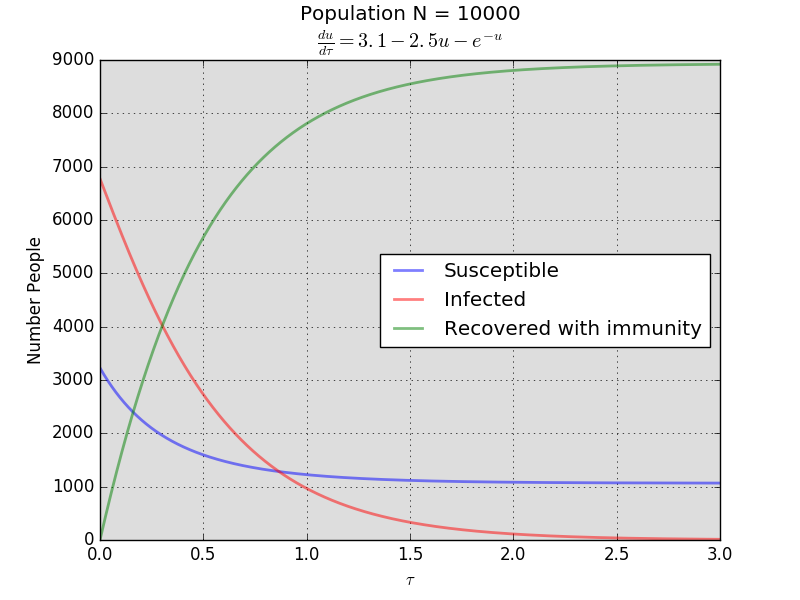
\includegraphics[width=1\textwidth]{q7_3.png}
\caption{\label{fig:data}Todo}
\end{figure}
\begin{figure}[H]
\centering
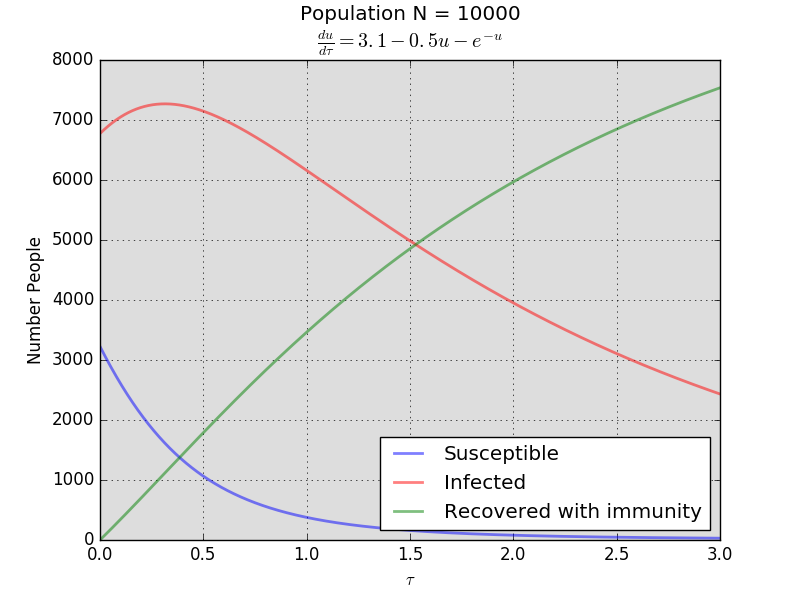
\includegraphics[width=1\textwidth]{q7_4.png}
\caption{\label{fig:data}Todo}
\end{figure}
\begin{figure}[H]
\centering
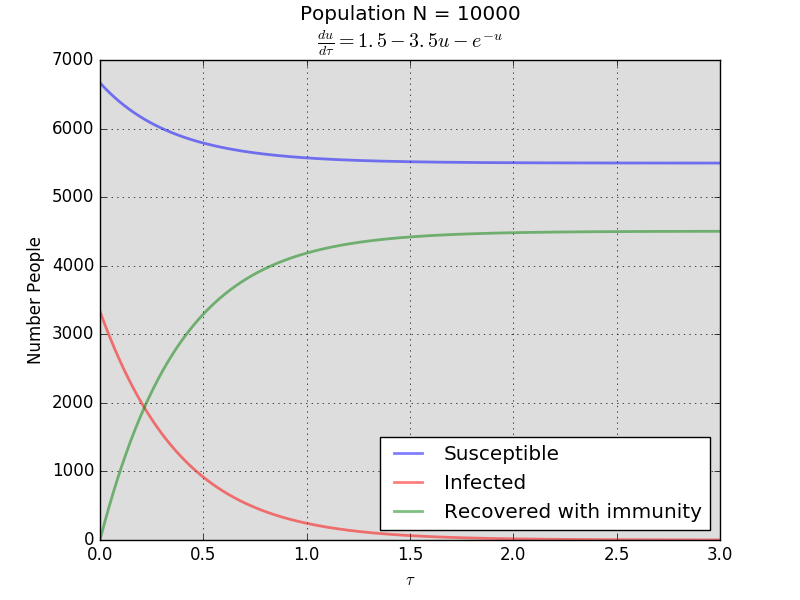
\includegraphics[width=1\textwidth]{q7_5.png}
\caption{\label{fig:data}Todo}
\end{figure}
\begin{figure}[H]
\centering
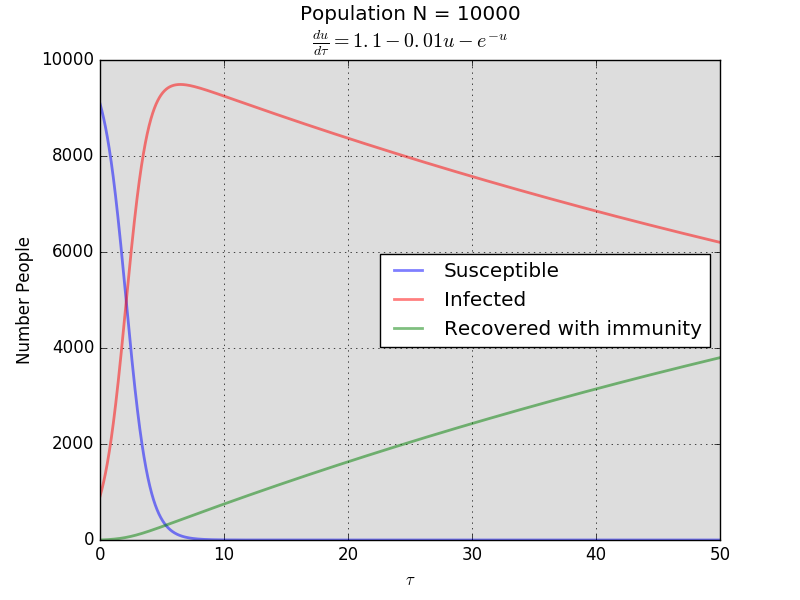
\includegraphics[width=1\textwidth]{q7_6.png}
\caption{\label{fig:data}Todo}
\end{figure}


\section{Full SIR model}

\begin{equation}
\begin{aligned}
F(x) &= -kxy + mz \\
G(y) &= kxy + ly \\
H(z) &= ly - mz 
\end{aligned}
\end{equation}

\subsection{Show $N = x + y + z$ is a constant}

\begin{align*}
\frac{\mathsf{d}N}{\mathsf{d}t} &= \frac{\mathsf{d}x}{\mathsf{d}t} + \frac{\mathsf{d}y}{\mathsf{d}t} + \frac{\mathsf{d}z}{\mathsf{d}t} \\
0 &= -kxy + mz + kxy + ly + ly - mz \\
0 &= 0  \\
\end{align*}

\subsection{Show $x = N, y = z = 0$ is  fixed point}

Substituting $x = N, y = z = 0$ in the Equations (2,3,4), yields

\begin{equation}
\frac{\mathsf{d}x}{\mathsf{d}t} = \frac{\mathsf{d}y}{\mathsf{d}t} = \frac{\mathsf{d}z}{\mathsf{d}t} = 0
\end{equation}

\subsection{Compute the Jacobian with the fixed point, Compute the eigenvalues of the Jacobian}

The jacobian associated with this system is defined as 

\[
J
=
\begin{bmatrix}
    \frac{\partial F_{x}}{\partial t} & \frac{\partial F_{y}}{\partial t} & \frac{\partial F_{z}}{\partial t} \\
    \frac{\partial G_{x}}{\partial t} & \frac{\partial G_{y}}{\partial t} & \frac{\partial G_{z}}{\partial t} \\
    \frac{\partial H_{x}}{\partial t} & \frac{\partial H_{y}}{\partial t} & \frac{\partial H_{z}}{\partial t} \\
\end{bmatrix}
= 
\begin{bmatrix}
    -ky & -kx & m \\
    ky & kx-l & m \\
    0 & l & -m \\
\end{bmatrix}
\]

Evaluating the jacobian at the fixed point $x = N, y = z = 0$
\[
J_{*}
= 
\begin{bmatrix}
    0 & -kN & m \\
    0 & kN-l & m \\
    0 & l & -m \\
\end{bmatrix}
\]

The eigenvalues in this case are the diagonal of $J_{*}$
\begin{align*}
 \lambda_{1} &= 0 \\
 \lambda_{2} &= kN - l \\
 \lambda_{3} &= -m 
\end{align*}

\subsection{Fixed point stability}

\begin{itemize}
 \item $\lambda_{1} = 0$ has no impact on the stability since it is neutral
 \item $\lambda_{3} = -m$ is stable as $m > 0$
 \item $\lambda_{2} = kN - l$ is stable if $kN < l$ and unstable if $kN > l$
\end{itemize}

For the fixed point to be stable, the infection rate $k$ would need to be very small relative to the recovery rate $l$

\begin{appendix}
   \newpage
   \addappheadtotoc
   \appendixpage
   \section{Python Code}
   \sloppy
   Python used to generate Figure (\ref{fig:3d})
   \lstinputlisting[language=Python,style=custom_py_style]{/home/ian/Desktop/ACM41000-Uncertainty-Quantification/assignment1/python-sandbox/figure1.py}
   Python used to generate Figure (\ref{fig:fp_diff_ab})
   \lstinputlisting[language=Python,style=custom_py_style]{/home/ian/Desktop/ACM41000-Uncertainty-Quantification/assignment1/python-sandbox/figure2.py}
   Python used to numerically solve the system of equations and generate Figures (4-9)
   \lstinputlisting[language=Python,style=custom_py_style]{/home/ian/Desktop/ACM41000-Uncertainty-Quantification/assignment1/python-sandbox/figure3.py}
   \section{Maxima Code}
   \sloppy
   Maxima command used to generate Figure (\ref{fig:df})
   \lstinputlisting[language=Python,style=custom_py_style]{/home/ian/Desktop/ACM41000-Uncertainty-Quantification/assignment1/df.maxima}
\end{appendix}


\end{document}
